

\tikzset{every picture/.style={line width=0.75pt}} %set default line width to 0.75pt        

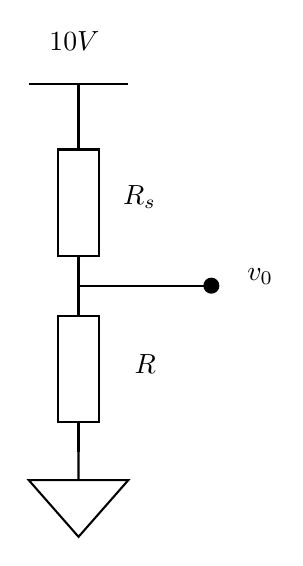
\begin{tikzpicture}[x=0.75pt,y=0.75pt,yscale=-1,xscale=1]

%Shape: Resistor [id:dp19596039193583614] 
\draw   (299,158.4) -- (299,209.6) -- (279,209.6) -- (279,158.4) -- (299,158.4) -- cycle (289,144) -- (289,158.4) (289,209.6) -- (289,224) ;
%Shape: Resistor [id:dp6717166589426362] 
\draw   (299,78.4) -- (299,129.6) -- (279,129.6) -- (279,78.4) -- (299,78.4) -- cycle (289,64) -- (289,78.4) (289,129.6) -- (289,144) ;
%Shape: Ground [id:dp8112994834936327] 
\draw   (265,237.67) -- (289,265) -- (313,237.67) -- (265,237.67) -- cycle (289,224) -- (289,237.67) ;
%Straight Lines [id:da6357261869016801] 
\draw    (289,144) -- (306,144) -- (353,144) ;
\draw [shift={(353,144)}, rotate = 0] [color={rgb, 255:red, 0; green, 0; blue, 0 }  ][fill={rgb, 255:red, 0; green, 0; blue, 0 }  ][line width=0.75]      (0, 0) circle [x radius= 3.35, y radius= 3.35]   ;
%Straight Lines [id:da11996191168558856] 
\draw    (265,47) -- (313,47) ;
%Straight Lines [id:da6468175768944302] 
\draw    (289,47) -- (289,64) ;

% Text Node
\draw (273.5,20.2) node [anchor=north west][inner sep=0.75pt]    {$10V$};
% Text Node
\draw (309,94.2) node [anchor=north west][inner sep=0.75pt]    {$R_{s} \ $};
% Text Node
\draw (368.8,134.4) node [anchor=north west][inner sep=0.75pt]    {$v_{0}$};
% Text Node
\draw (314.5,175.8) node [anchor=north west][inner sep=0.75pt]    {$R$};


\end{tikzpicture}
